\documentclass[11pt,dvipsnames,svgnames]{report}

%PRÉAMBULE
\usepackage[french]{babel}
\usepackage[utf8]{inputenc}
%\usepackage[table]{xcolor}
\usepackage[T1]{fontenc}
\usepackage[normalem]{ulem}
\usepackage{verbatim}
\usepackage{fancyhdr}
\usepackage{mdframed}
%\usepackage{xcolor}
\usepackage{graphicx}
\usepackage{fancybox}
\usepackage{amsfonts}
\usepackage{amsmath}
\usepackage{ulem}
\usepackage{eurosym}
\usepackage{float}
\usepackage{adjustbox}
\usepackage{amssymb,amsmath,latexsym}
\usepackage{mathrsfs}
\usepackage[a4paper]{geometry}
\usepackage[bottom]{footmisc}
\usepackage{perpage}
\usepackage{multicol}
\PassOptionsToPackage{hyphens}{url}
\usepackage[breaklinks]{hyperref}
\usepackage[final]{pdfpages}
\usepackage{appendix}
\usepackage{caption}
\usepackage{minitoc}
%\usepackage{tikz}
\usepackage{listings}
\usepackage{setspace}
\usepackage{titlesec}
\usepackage{float}
\usepackage[section]{placeins}
\usepackage{rotating}
\usepackage{subfigure}
\usepackage{epsfig}
%\usepackage{mathpazo}
%\usepackage[scaled]{beramono}
\usepackage{menukeys}
\usepackage{etoolbox}
\makeatletter
\patchcmd{\ttlh@hang}{\parindent\z@}{\parindent\z@\leavevmode}{}{}
\patchcmd{\ttlh@hang}{\noindent}{}{}{}
\makeatother


\geometry{hmargin=2.5cm,vmargin=2cm}

\definecolor{dkgreen}{rgb}{0,0.6,0}
\definecolor{gray}{rgb}{0.5,0.5,0.5}
\definecolor{mauve}{rgb}{0.58,0,0.82}
\definecolor{darkblue}{rgb}{0.0,0.0,0.6}
\definecolor{cyan}{rgb}{0.0,0.6,0.6}

\lstset{frame=tb,
  language=Java,
  aboveskip=3mm,
  belowskip=3mm,
  showstringspaces=false,
  columns=flexible,
  basicstyle={\footnotesize\ttfamily},
  numbers=none,
  numberstyle=\tiny\color{gray},
  keywordstyle=\color{blue},
  commentstyle=\color{dkgreen},
  stringstyle=\color{mauve},
  breaklines=false,
  breakatwhitespace=true,
  tabsize=3
}


\setcounter{secnumdepth}{4}
\setcounter{tocdepth}{4}


% En-têtes et pieds-de-page
\pagestyle{fancy}
\renewcommand\headrulewidth{1pt}
\fancyhead[L]{\small{\leftmark}}
\fancyhead[R]{
\includegraphics[scale=0.2]{images/logoasi.png}}
\fancyhfoffset{0pt}
\fancyfoot[R]{\setstretch{0,8}\small{GD, AH, MJ, RJ, AL}}
\fancyfoot[L]{
\includegraphics[scale=0.14]{images/LogoINSA.png}}
\renewcommand{\headrule}{{%
 \color{black}\hrule \headwidth \headrulewidth \vskip-\headrulewidth}}
\titleformat{\section}%
[hang]% style du titre (hang, display, runin, leftmargin, drop, wrap)
{\Large\bfseries}%changement de fonte commun au numéro et au titre
{\thesection}% spécification du numéro
{1em}% espace entre le numéro et le titre
{}% changement de fonte du titre


\begin{document}

\begin{titlepage}
\newcommand{\HRule}{\rule{\linewidth}{0.5mm}}
\center
\vspace*{\stretch{1}}\textsc{\huge INSA Rouen Normandie}\\[0.7cm]
\LARGE Département ASI~\\[0.5cm]
\Large{4ème année} ~\\[1.5cm]
\textsc{\Large EC Informatique Répartie}\\[0.5cm]

\HRule \\[0.4cm]
{ \huge \bfseries Messagerie instantanée 1}\\[0.18cm] \HRule \\[1.5cm]

\LARGE \emph{\textbf{Rapport de projet}} \\[1.3cm]

\large
	\emph{\textbf{Auteurs}}\\
	Gautier \textsc{Darchen} \\
	Alexandre \textsc{Huat} \\
	Marie-Andrée \textsc{Jolibois} \\
	Romain \textsc{Judic} \\
	Alexandre \textsc{Le Lain}\\[0.3cm]

\vfill{\today}

\begin{figure}

\includegraphics[width=4cm]{images/LogoINSA.png}\hfill

\includegraphics[width=3cm]{images/logoasi.png}
\end{figure}

%----------------------------------------------------------------------------------------

\vspace*{\stretch{1}}
 \end{titlepage}

\newpage
\tableofcontents

\newpage


\chapter{Introduction}

L'application à développer est une plateforme graphique répartie de messagerie instantanée. 


\section{Fonctions principales}
Les fonctions principales de cette application peuvent être scindées en trois catégories :
\begin{itemize}
\item l'échange de messages ;
\item le filtrage des messages en fonction de leur contenu ;
\item l'utilisation d'un avatar.
\end{itemize}

Concernant la première fonctionnalité, les interlocuteurs pourront s'envoyer des messages écrits de façon instantanée. Ils auront en plus la possibilité de communiquer avec d'autres formats via un système de visio- ou audio-conférence intégré à l'application.

Le filtrage des messages prend en charge le contrôle parental et la modération. Les utilisateurs auront la possibilité de choisir d'activer ou non ce système de filtrage. De plus, ce dernier pourra être personnalisé.

Concernant la dernière fonctionnalité, un système d'avatar pourra être utilisé par les utilisateurs pour les conversations audio et écrites.


\section{Utilisateurs}
Il existe plusieurs types d'utilisateurs.
\begin{description}
\item[Utilisateur \emph{lambda} :] il peut créer (ouvrir) une conversation, participer à une conversation qu'il sélectionne. Il peut paramétrer ses filtres. À la connexion, il choisit aussi un login et un avatar.
\item[Modérateur :] il peut émettre des messages de modération et supprimer des messages d'utilisateurs.
\end{description}
\vskip \baselineskip

\begin{mdframed}[topline=false,rightline=false,bottomline=false, linewidth=3pt,linecolor=red]
Plusieurs utilisateurs peuvent discuter en même temps sur une même conversation.
\end{mdframed}

Les seuls prérequis à l'utilisation sont savoir exécuter des lignes de commandes pour installer et exécuter une application.
\section{Contraintes}
\subsection{Contraintes matérielles}
L'utilisateur doit disposer d'une machine reliée à internet.

Pour profiter du service visio, l'utilisateur doit posséder un matériel de capture vidéo (webcam) et d'entrées/sorties audio.

Pour utiliser le service audio, l'utilisateur doit posséder une entrée et une sortie audio.

La majorité des calculs est réalisée côté serveur, ce qui n'implique pas un besoin de ressources conséquentes côté client.

\subsection{Contraintes logicielles}

Le client doit disposer du Java Runtime Environnement 8 et de la bibliothèque JavaFX.\\

Installer JavaFX en ligne de commande sous Ubuntu 16.04+ :

\begin{lstlisting}
sudo apt-get update
sudo apt-get install openjfx
\end{lstlisting}

\chapter{Spécifications}

\section{Spécifications fonctionnelles}

\begin{mdframed}[topline=false,rightline=false,bottomline=false, linewidth=3pt,linecolor=red]
~\\\indent Les comptes utilisateurs ne sont pas persistants, ils n'existent que de l'ouveture à la fermeture d'un service client. L'utilisateur peut paramétrer son compte (pseudo et avatar) avant de participer à une conversation.

Les utilisateurs modérateurs peuvent supprimer des messages.

Tout utilisateur peut ouvrir ou rejoindre une conversation. Les conversations existent indépendamment des utilisateurs, elles sont ouvertes aussi longtemps que le serveur les hébergeant est actif.

L'IA est un helpbot présent sur chaque conversation. L'utilisateur peut l'invoquer en entrant des mots clés commençant pas un backslash.
\begin{description}
\item[\textbackslash bonjour] salue l'utilisateur et déroule un menu d'aide.
\item[\textbackslash profil] indique à l'utilisateur comment paramétrer son profil.
\item[\textbackslash filtre] indique à l'utilisateur comment paramétrer les filtres.
\item[\textbackslash chat1] indique à l'utilisateur comment ouvrir une conversation.
\item[\textbackslash chat2] indique à l'utilisateur comment rejoindre une conversation.
\item[\textbackslash video] indique à l'utilisateur comment démarrer une conversation vidéo.
\item[\textbackslash audio] indique à l'utilisateur comment démarrer une conversation audio.
\end{description}


\end{mdframed}

\subsection*{Cas d'utilisation}

Cette section présente les cas d'utilisation suivants :
\begin{itemize}
\item discuter ;
\item paramétrer le filtrage ;
\item filtrer les messages ;
\item se connecter.
\end{itemize}

\begin{figure}[H]
\caption{Cas d'utilisation \textbf{discuter}}
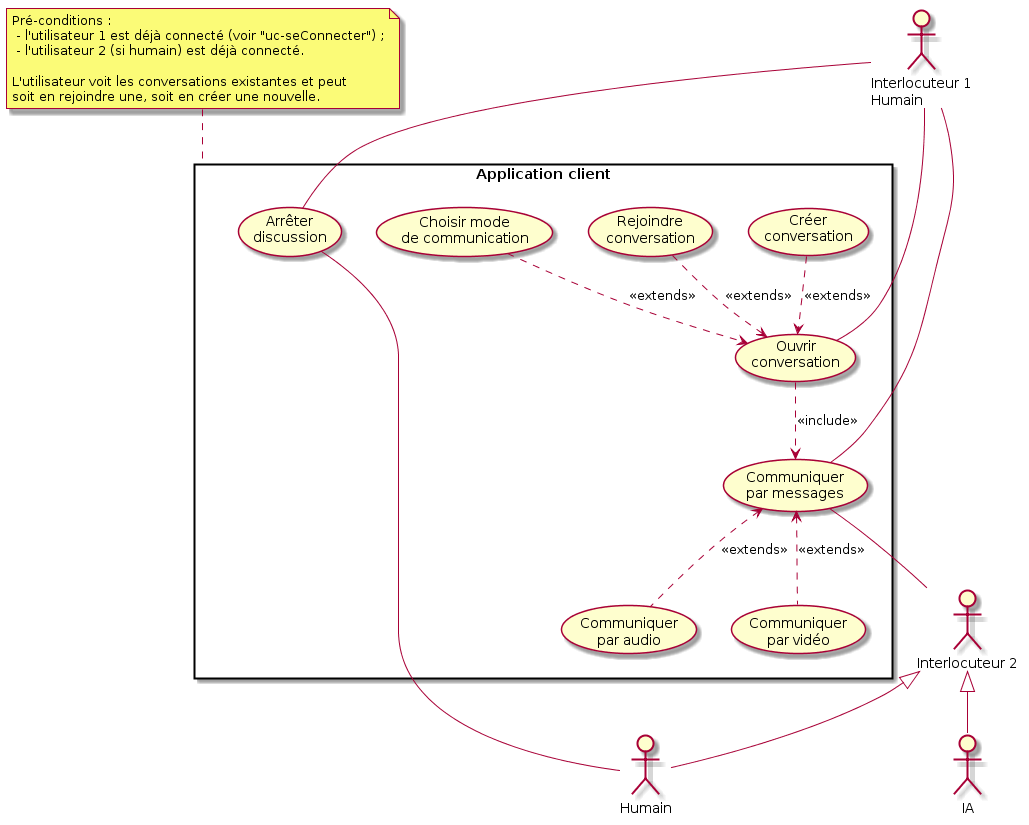
\includegraphics[width=\linewidth]{images/uc-discuter.png}
\label{cas1}
\end{figure}
Le cas d'utilisation (figure \ref{cas1}) représente les interactions entre les différents interlocuteurs et les différents moyens mis à leur disposition pour communiquer.

\begin{center}
\begin{figure}[H]
\caption{Cas d'utilisation \textbf{filtrer les messages}}
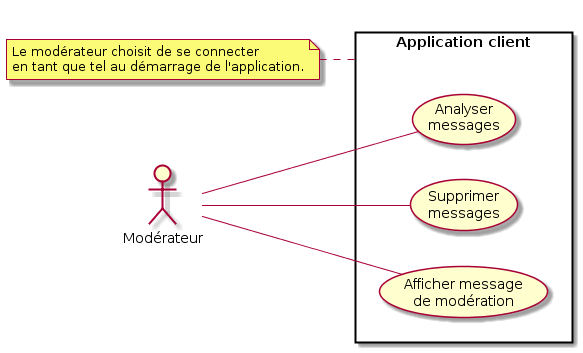
\includegraphics[width=\linewidth]{images/uc-filtrerMessages.png}
\end{figure}

\begin{figure}
\caption{Cas d'utilisation \textbf{paramétrer le filtrage}}
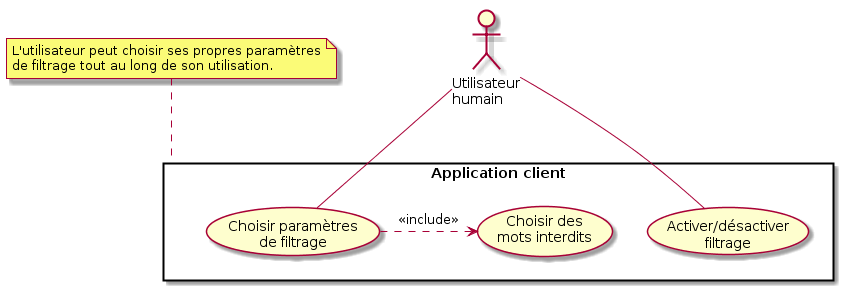
\includegraphics[width=\linewidth]{images/uc-parametrerFiltrage.png}
\end{figure}

\begin{figure}
\caption{Cas d'utilisation \textbf{se connecter}}
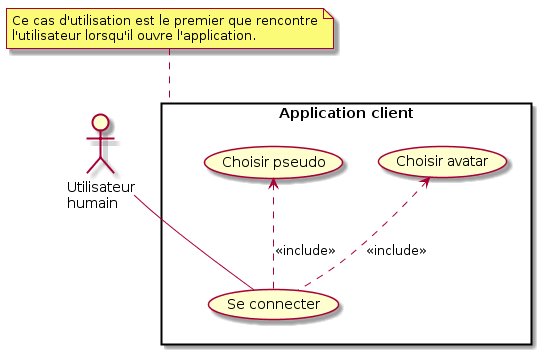
\includegraphics[width=\linewidth]{images/uc-seConnecter.png}
\end{figure}

\end{center}

\section{Spécifications d'interfaces}
\subsection*{Maquettes}

Cette section présente les maquettes de l'application.

\begin{figure}[H]
\caption{Exemple de conversation texte}
\centerline{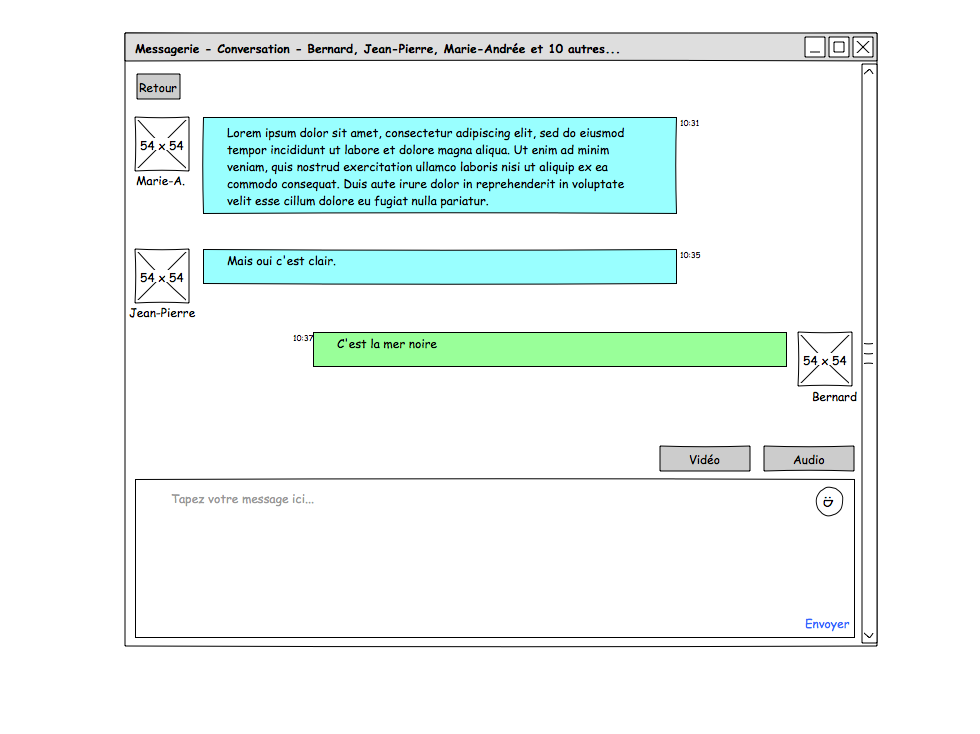
\includegraphics[width=.9\linewidth]{maquette/maquette1.png}}
\end{figure}

\begin{figure}[H]
\caption{Conversation vidéo}
\centerline{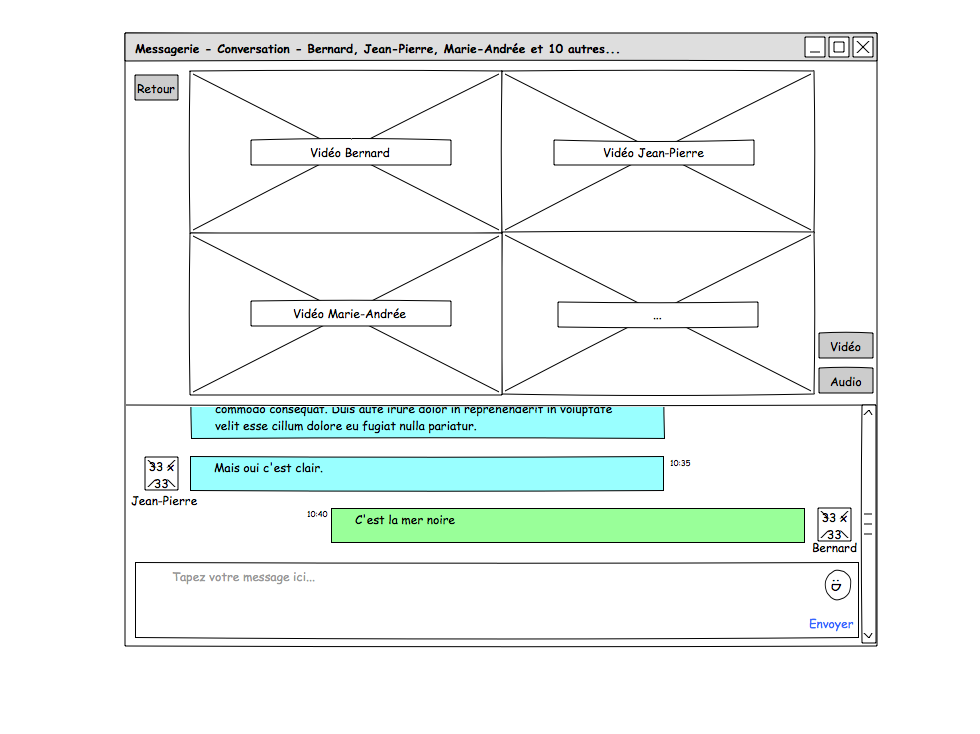
\includegraphics[width=0.9\textwidth]{maquette/maquette4.png}}
\end{figure}

\begin{figure}[H]
\caption{Liste des conversations}
\centerline{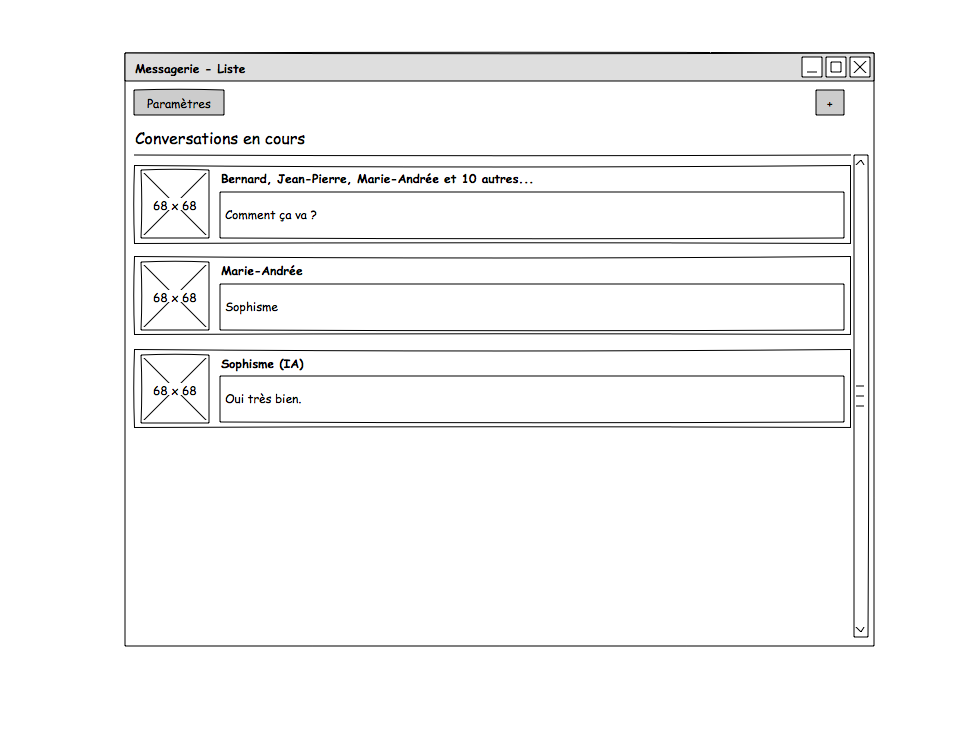
\includegraphics[width=0.9\textwidth]{maquette/maquette2.png}}
\end{figure}

\begin{figure}[H]
\caption{Interface des paramètres}
\centerline{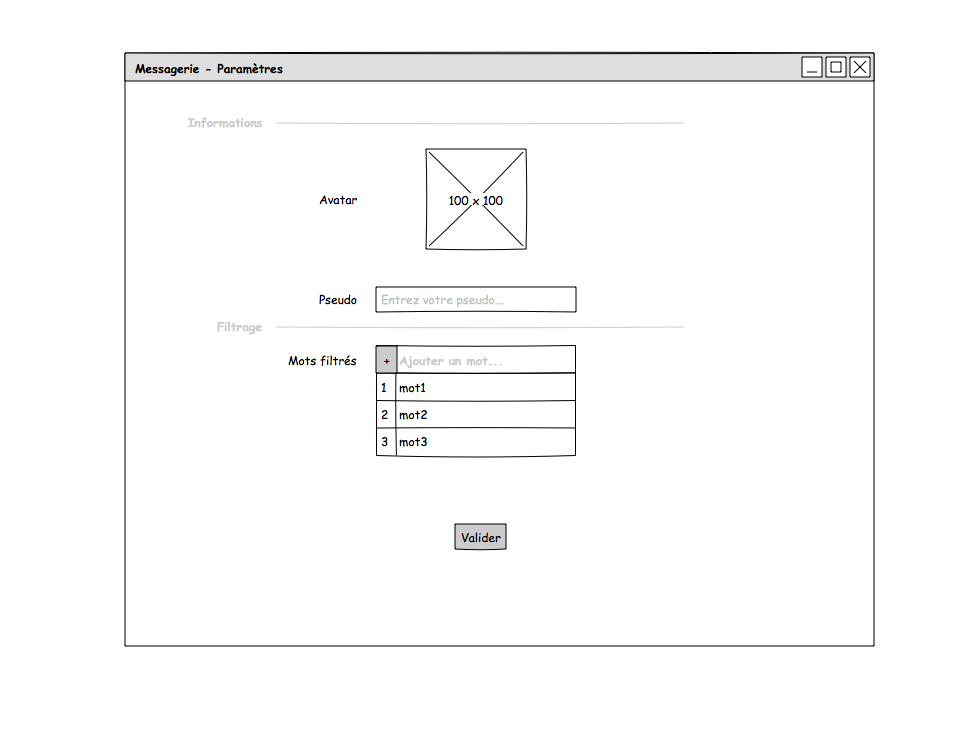
\includegraphics[width=0.9\textwidth]{maquette/maquette3.png}}
\end{figure}


\section{Spécifications opérationnelles}

Le système de messagerie répond instantanément.

Les messages sont sauvegardés tant qu'il subsiste un utilisateur connecté à la conversation.

Tant que le serveur est actif, le service client est disponible.

Lors de l'utilisation de l'application, la référence du compte est utilisée pour savoir qui participe à la conversation. Cette référence du compte transite donc entre l'application client et l'application serveur. Aucune mesure de sécurité n'est prévue pour éviter une transmission visible de cette référence.\\

\chapter{Conception préliminaire}

\section{Modèle du domaine}

\begin{figure}[H]
\caption{Modèle du domaine}
\centerline{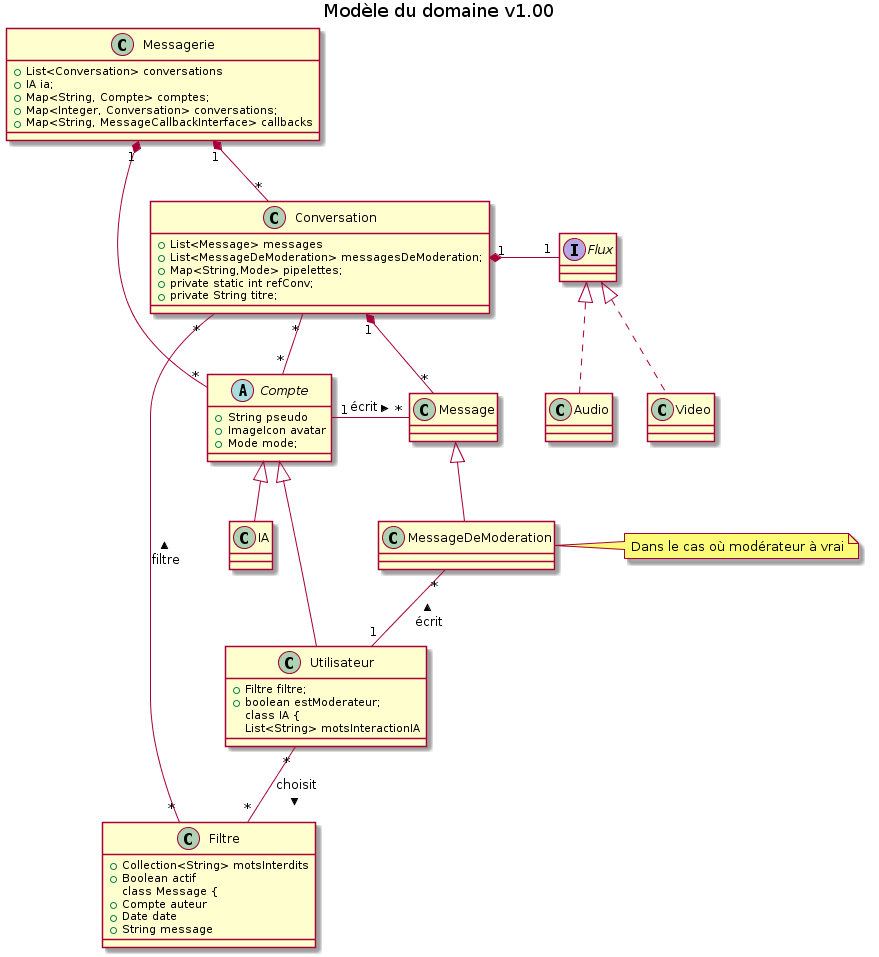
\includegraphics[width=0.95\textwidth]{diagrammes/class-diag.png}}
\end{figure}

\section{Diagrammes de séquence système}

\begin{figure}[H]
\caption{Diagramme de séquence système de \textbf{communiquer}}
\centerline{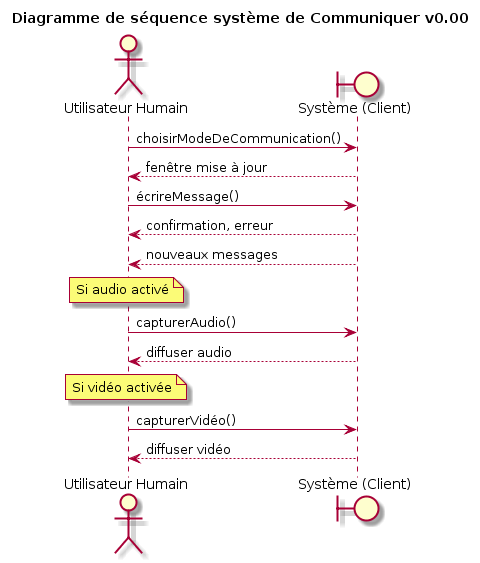
\includegraphics[width=0.9\textwidth]{diagrammes/dss-communiquer.png}}
\end{figure}

\begin{figure}[H]
\caption{Diagramme de séquence système de \textbf{se connecter}}
\centerline{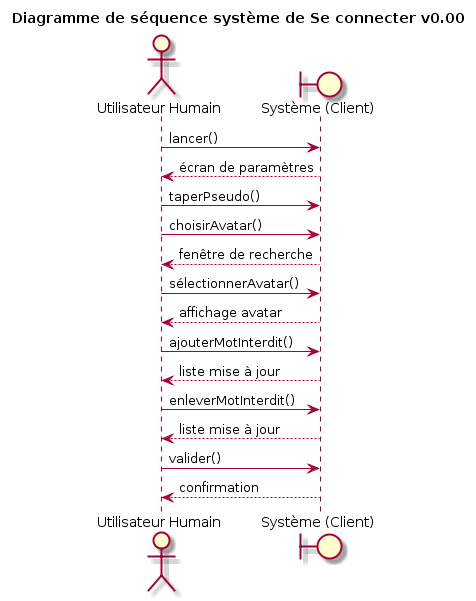
\includegraphics[width=0.9\textwidth]{diagrammes/dss-connexion.png}}
\end{figure}

\begin{figure}[H]
\caption{Diagramme de séquence système de \textbf{modérer}}
\centerline{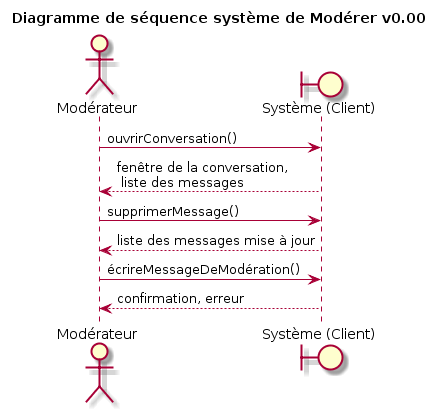
\includegraphics[width=0.9\textwidth]{diagrammes/dss-moderer.png}}
\end{figure}

\subsection{Modification du modèle du domaine}
\begin{itemize}
\item Ajout d'attributs dans la classe \texttt{Messagerie}.
\item L'interface \texttt{Moderateur} est remplacé par un attribut booléen de la classe \texttt{Utilisateur}.
\end{itemize}

\section{Diagrammes d'activités}
\begin{figure}[H]
\caption{Diagramme d'activité de \textbf{se connecter}}
\centerline{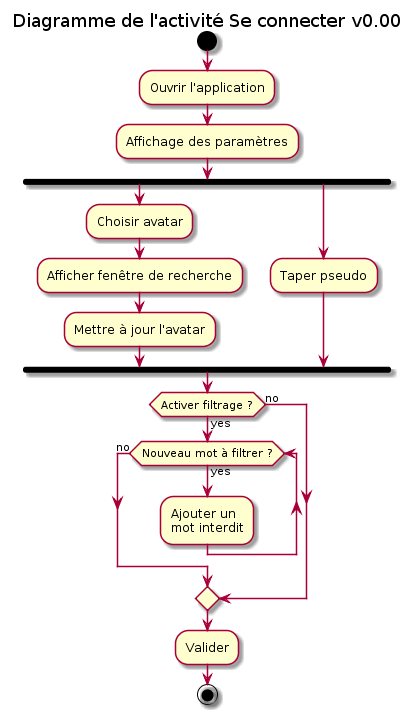
\includegraphics[width=0.75\textwidth]{diagrammes/activity-settings-diag.png}}
\end{figure}

\begin{figure}[H]
\caption{Diagramme d'activité de \textbf{choisir une conversation}}
\centerline{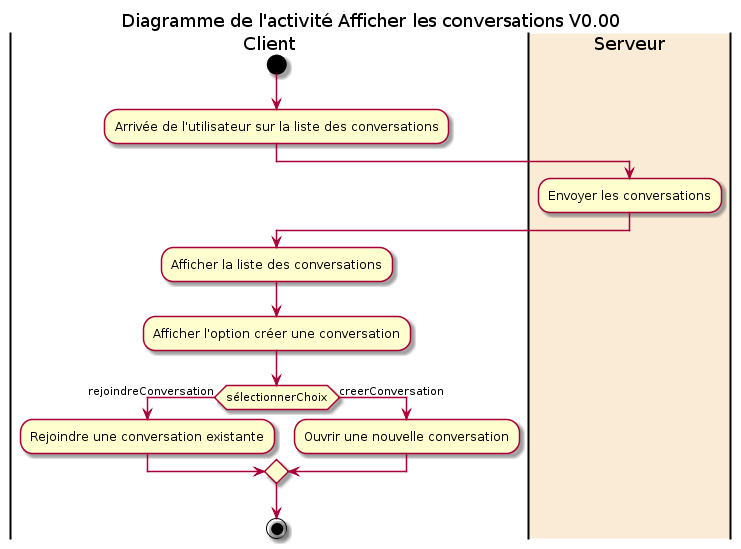
\includegraphics[width=0.95\textwidth]{diagrammes/activity-convList-diag.png}}
\end{figure}

\begin{figure}[H]
\caption{Diagramme d'activité d'\textbf{ouvrir une conversation}}
\centerline{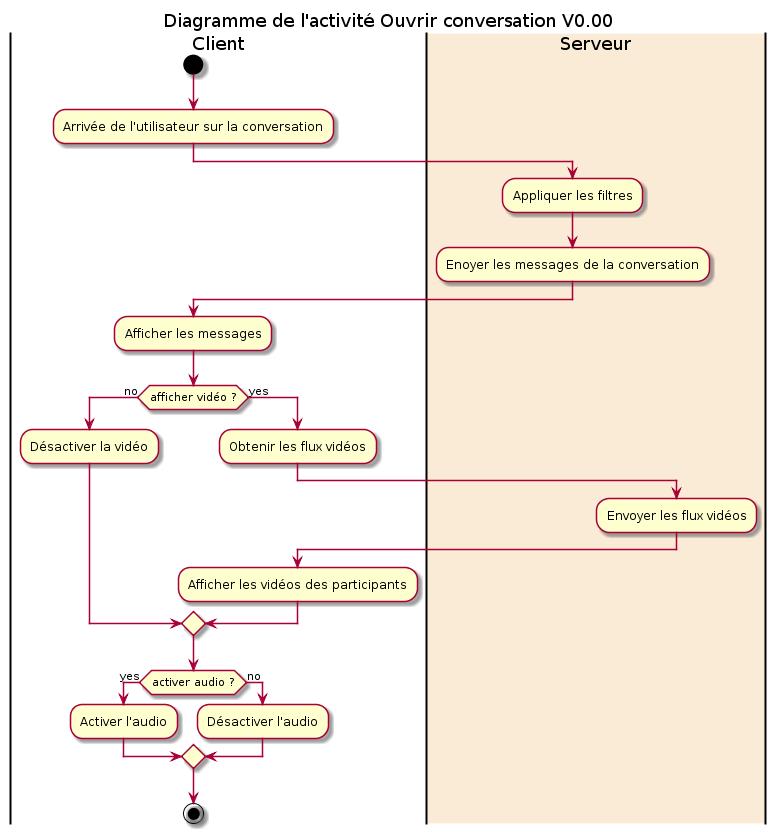
\includegraphics[width=0.75\textwidth]{diagrammes/activity-openConv-diag.png}}
\end{figure}

\begin{figure}[H]
\caption{Diagramme d'activité de \textbf{communiquer}}
\centerline{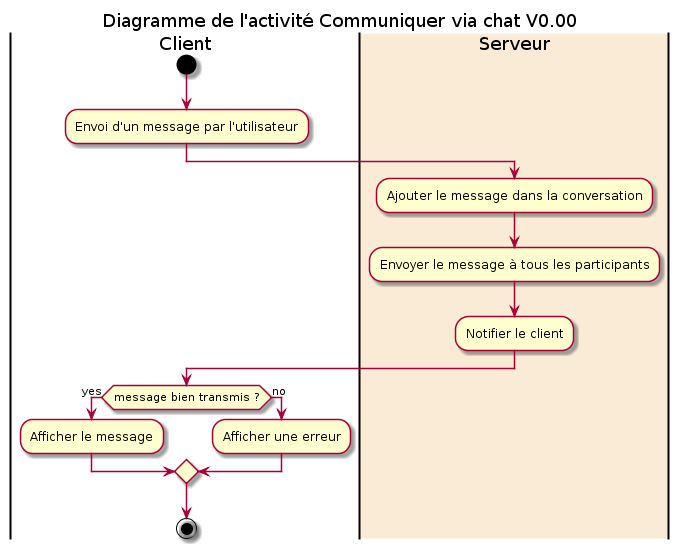
\includegraphics[width=0.8\textwidth]{diagrammes/activity-sendMsg-diag.png}}
\end{figure}

\section{Diagrammes d’interaction}

\begin{figure}[H]
\caption{Diagramme de séquence d'analyse de \textbf{se connecter}}
\centerline{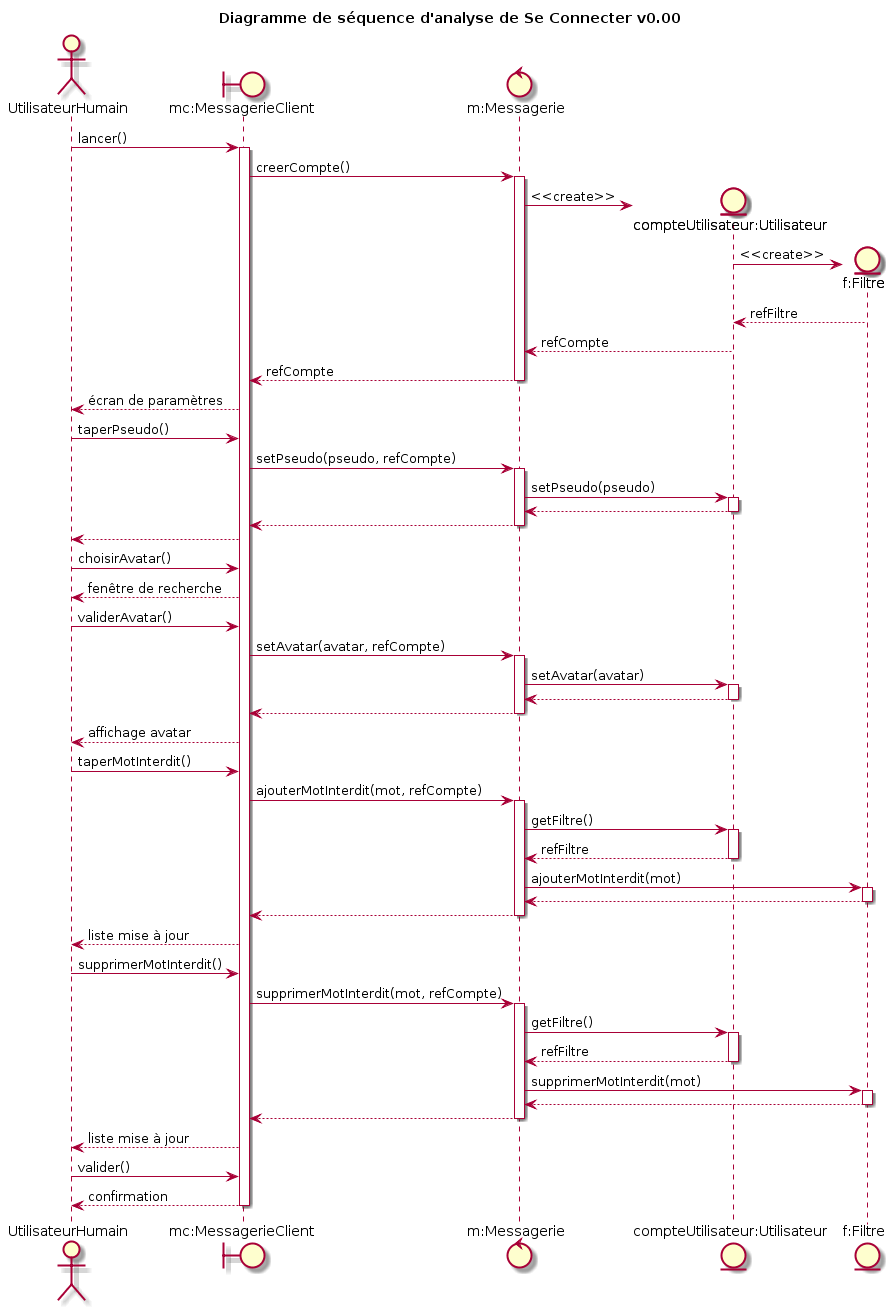
\includegraphics[width=\textwidth]{diagrammes/dsa-connexion.png}}
\end{figure}

\begin{figure}[H]
\caption{Diagramme de séquence d'analyse de \textbf{communiquer}}
\centerline{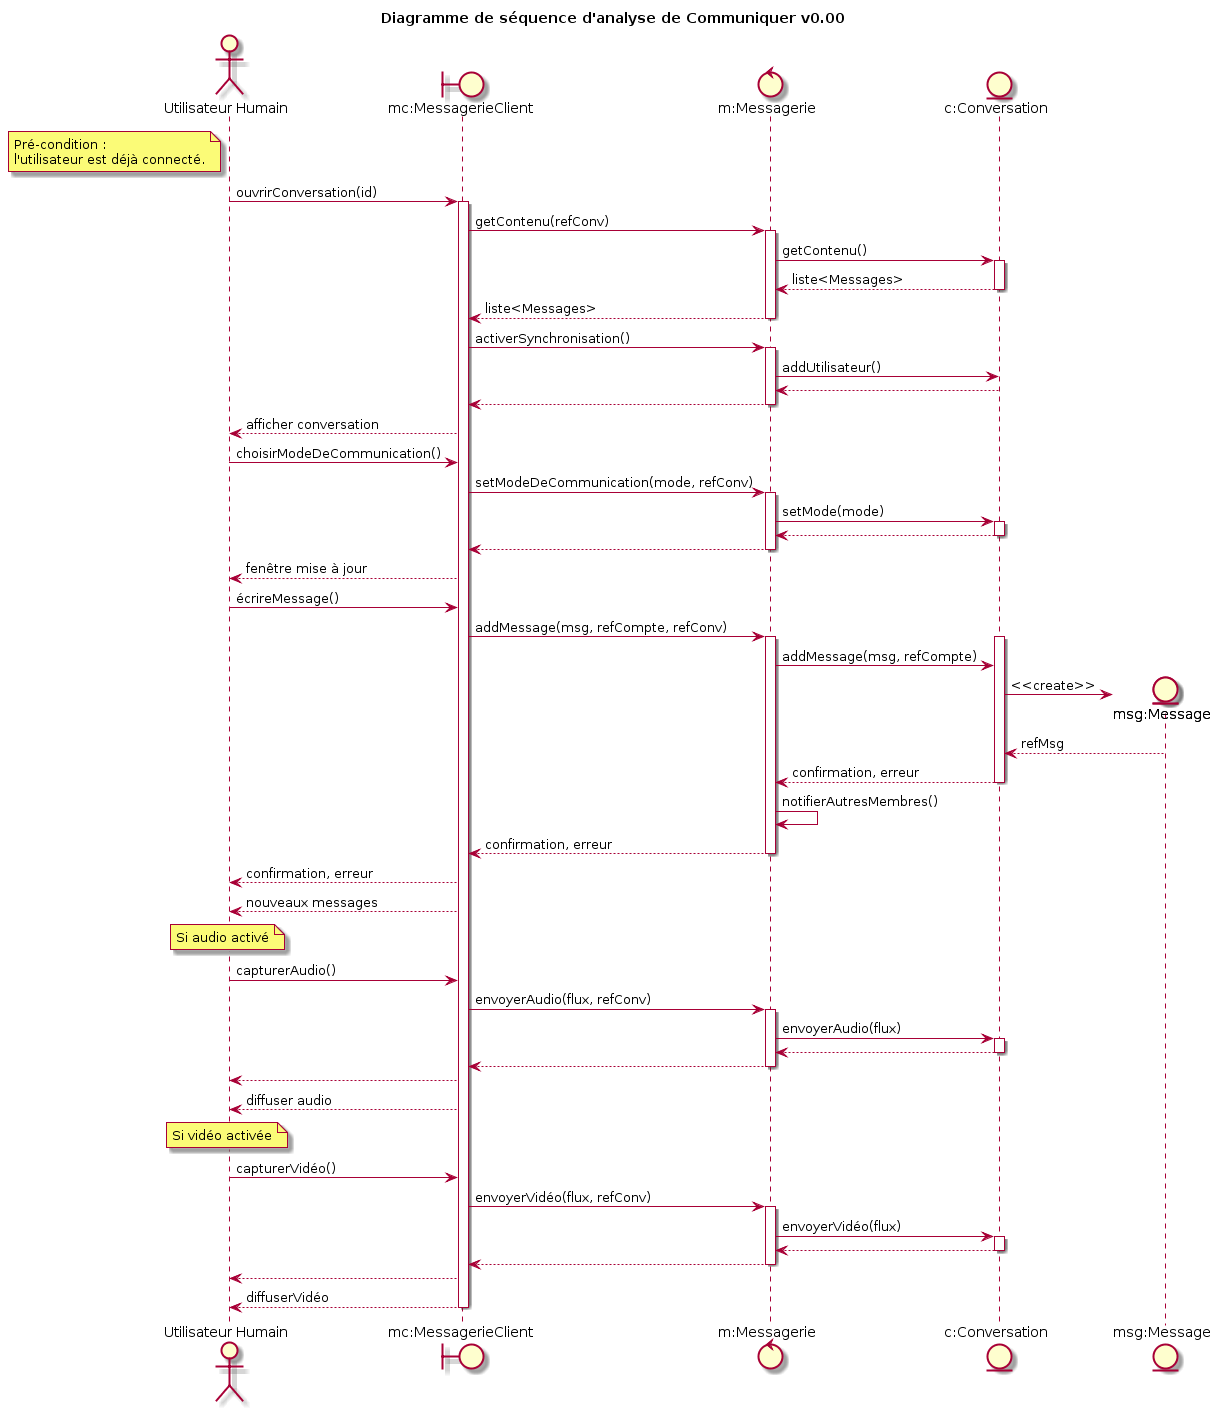
\includegraphics[width=\textwidth]{diagrammes/dsa-communiquer.png}}
\end{figure}

\begin{figure}[H]
\caption{Diagramme de séquence d'analyse de \textbf{modérer un message}}
\centerline{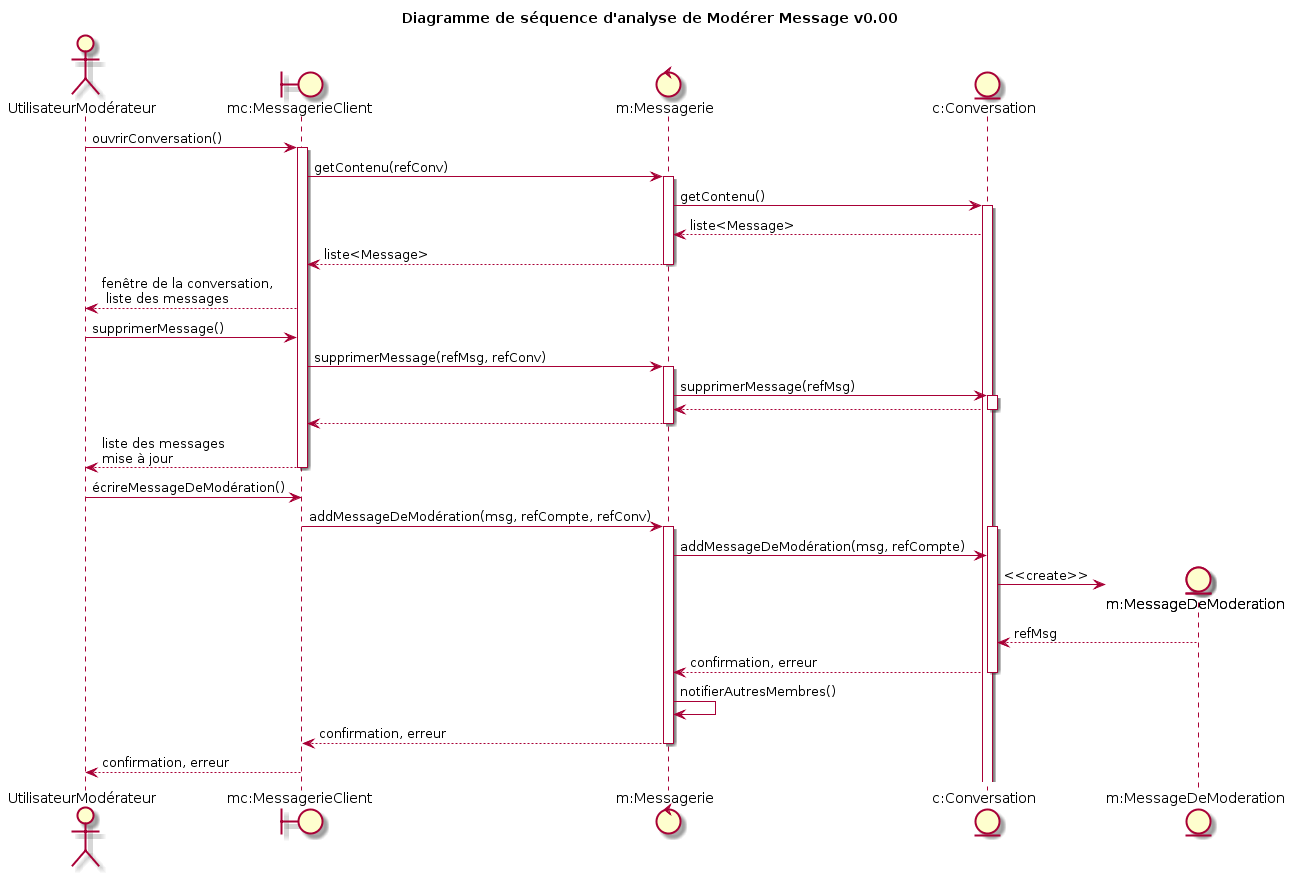
\includegraphics[width=\textwidth]{diagrammes/dsa-moderer.png}}
\end{figure}

\newpage
\section{Découpage de l'application en \emph{packages}}
\begin{figure}[H]
\caption{Diagramme de packages}
\centerline{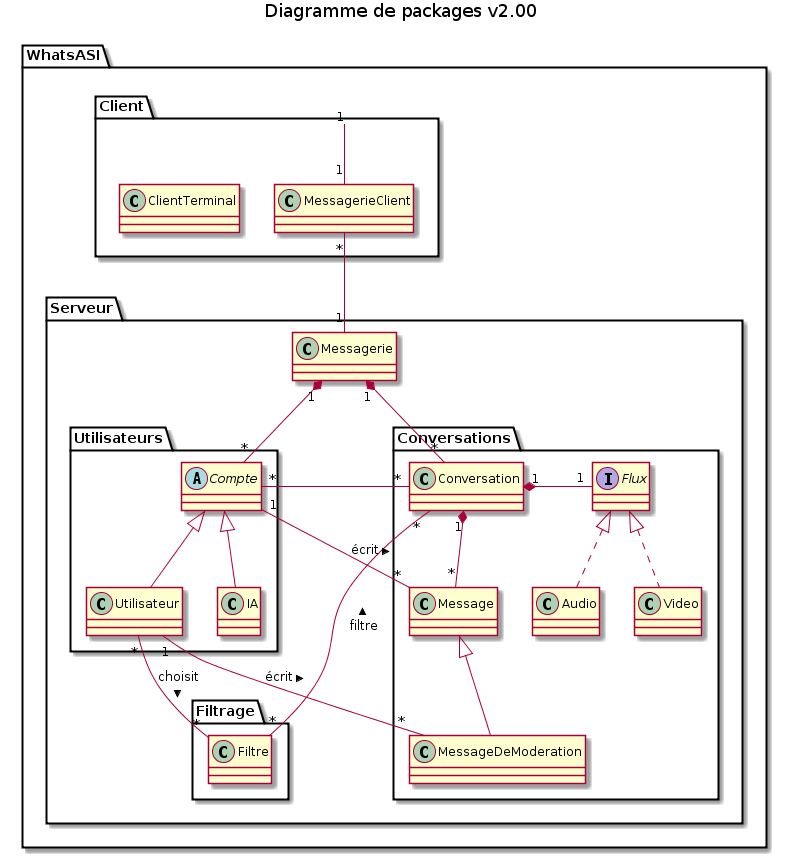
\includegraphics[width=0.8\textwidth]{diagrammes/package-diag.png}}
\end{figure}


%\paragraph*{Classe Messagerie}
%\begin{itemize}
%\item \texttt{public List<Conversation> getConversations()} ;
%\end{itemize}
%
%\paragraph*{Classe Conversation}
%\begin{itemize}
%\item \texttt{public List<Message> getMessages()} ;
%\item \texttt{public List<Compte> getListeParticipants()} ;
%\item \texttt{public void afficherConversation()} ;
%\item \texttt{public void supprMessageInList(Message msg)} ;
%\item \texttt{public void broadcastInMsg()} ;
%\item \texttt{public void addMessageInList(Message msg)} ;
%
%\end{itemize}
%
%\paragraph*{Interface Video}
%\begin{itemize}
%\item \texttt{public void startVideo()} ;
%\item \texttt{public void endVideo()} ;
%\end{itemize}
%
%\paragraph*{Interface Audio}
%\begin{itemize}
%\item \texttt{public void startAudio()} ;
%\item \texttt{public void endAudio()} ;
%\end{itemize}
%
%\paragraph*{Classe Message}
%\begin{itemize}
%\item \texttt{public Compte getAuteur()} ;
%\item \texttt{public Date getDate()} ;
%\item \texttt{public String getMessage()} ;
%\end{itemize}
%
%\paragraph*{Classe MessageDeModeration}
%\begin{itemize}
%\item \texttt{public void sendMessageDeModeration(String message)} ;
%
%\end{itemize}
%
%\subsubsection{\og Gestion des utilisateurs \fg}
%
%\paragraph*{Classe Abstraite Compte}
%\begin{itemize}
%\item \texttt{public String getPseudo()} ;
%\item \texttt{public ImageIcon getAvatar()} ;
%\item \texttt{public boolean canVideo()} ;
%\item \texttt{public boolean canAudio()} ;
%\item \texttt{public void setVideo(boolean b)} ;
%\item \texttt{public void setAudio(boolean b)} ;
%\end{itemize}
%
%\paragraph*{Classe Moderateur}~\\
%Hérite de la classe abstraite \texttt{Compte}.
%\begin{itemize}
%\item \texttt{public void selectionnerConversation()} ;
%\item \texttt{public bool supprimerMessage(Message msg)} ;
%\item \texttt{public void messageDeModeration(Message msg)} ;
%\end{itemize}
%
%\paragraph*{Classe IA}~\\
%Hérite de la classe abstraite \texttt{Compte}.
%\begin{itemize}
%\item \texttt{public Collection<String> getMessagesPossiblesIA()} ;
%\item \texttt{public String answerMessage(String messageRecu)} ;
%\end{itemize}
%
%\paragraph*{Classe Utilisateur}~\\
%Hérite de la classe abstraite \texttt{Compte}.
%\begin{itemize}
%\item \texttt{public Filtre getFiltre()} ;
%\item \texttt{public void selectionModificationDeCompte()} ;
%\item \texttt{public void modifierAvatar()} ;
%\item \texttt{public void selectionImage()} ;
%\item \texttt{public void modifierPseudo()} ;
%\end{itemize}
%
%
%\subsubsection{\og Gestion du filtrage \fg}
%
%\paragraph*{Classe Filtre}
%\begin{itemize}
%\item \texttt{public Collection<String> getMotsInterdits()} ;
%\item \texttt{public void addMotInterdit(String mot)} ;
%\end{itemize}
%

\chapter{Conception détaillée}
\begin{figure}[H]
\caption{Diagramme de classes de conception détaillée}
\centerline{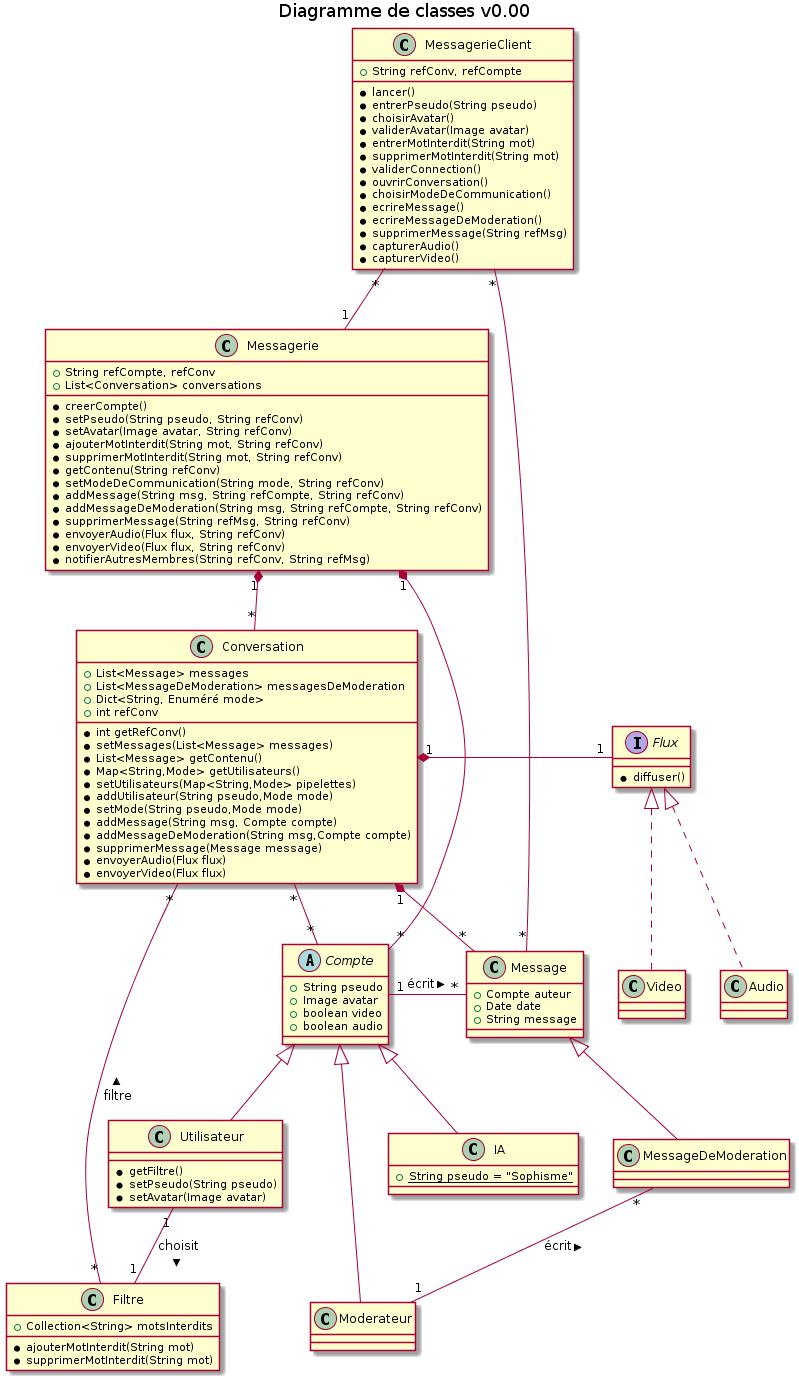
\includegraphics[height=18cm]{diagrammes/detailedConception.png}}
\end{figure}
\chapter{Implémentations et tests}
Cette partie précise et justifie nos choix techniques et restitue les résultats des tests de validation.
\section{Choix techniques}
\subsection{Langage de programmation}
Nous avons réaliser toute l'application en Java car ce langage est connu de toute l'équipe et permettait une implémentation rapide des technologies d'informatique répartie apprises avant le projet.
\subsection{Bibliothèques}
Le client graphique est une application JavaFX. L'ensemble de l'équipe avait été initiée à Swing en ASI3 mais JavaFX est la bibliothèque graphique officielle de Java depuis la sortie de la Java SE 8 en 2014. Se tenir à jour sur les dernières technologies justifiait ce choix.
\subsection{Technologie répartie}
Nous avons choisi la technologie d'informatique répartie RMI, plutôt que REST par exemple, car nous avons réalisé un logiciel non Web.
\subsection{Difficultés}
La prise en main de JavaFX n'a pas été aisée, en particulier la manipulation des \texttt{ListView} qui sont des objets graphiques permettant de visualiser une liste d'éléments (des messages dans une conversation, ici).

Aussi, le fait que la mise à jour des éléments graphiques de JavaFX est asynchrone et difficilement forçable a parfois posé problème sur la mise à jour des conversations qui ne se faisait pas en temps réel selon l'ordinateur.

Nous avons également été confronté à un problème de sérialisation avec les images. En effet, dans toute la Java SE 8, seule la classe d'image \texttt{IconImage} est sérialisable. Mais la taille d'une image ne peut être sauvegardée, cela a donc posé des problèmes d'affichage (de \emph{resizing}) que nous avons résolus en imposant le choix d'avatars à taille fixe.

Enfin, la fonction de \emph{callback} permettant la mise à jour des conversations côté client à chaque évènement côté serveur n'était pas une partie facile.
\subsection{Guide d'utilisation}
\paragraph*{Installation/Exécution}
\begin{enumerate}
\item Compilez le projet via le fichier \texttt{compile.sh}.
\begin{lstlisting}
   ./compile.sh
\end{lstlisting}
\item Lancez le RMIRegistry.
\begin{lstlisting}
   ./launchRmiregistry.sh
\end{lstlisting}
\item Lancez le serveur (dans un autre terminal).
\begin{lstlisting}
   ./launchServer.sh
\end{lstlisting}
\item Lancez le client graphique (dans un autre terminal).
\begin{lstlisting}
   ./launchClient.sh 
\end{lstlisting}
\item ... ou en ligne de commande.
\begin{lstlisting}
   ./launchClient.sh terminal
\end{lstlisting}
\end{enumerate}

\paragraph*{Utilisation}
L'IHM est intuitive.

\begin{enumerate}
\item Choisissez un avatar et un pseudo sur le panneau de connexion et cliquez sur \menu{Se connecter}.
\item Un panneau s'ouvre. Saisissez des mots à filtrer dans les conversations.
\item Le panneau des conversations s'ouvre. Créez une nouvelle conversation en cliquant sur \menu{+} et cliquez sur un titre de conversation dans la barre latérale. Vous pouvez maintenant envoyer des messages comme dans n'importe d'autre application standards.
\item Les informations détaillées sont fournies par l'IA d'aide, invocable en écrivant \texttt{\textbackslash bonjour} dans n'importe quelle conversation.
\end{enumerate}

\paragraph*{Exemples d'utilisation}
La figure \ref{illuConn} illustre la connexion d'un utilisateur modérateur.

La figure \ref{illuFiltre} illustre le paramétrage des filtres de ce même utilisateur.

La figure \ref{illuConv} illustre une conversation entre deux utilisateurs dont celui de gauche, A. Pauchet, a filtré le mot \og 20 \fg{}. On constate sur la fenêtre de droite, du modérateur, que celui-ci peut supprimer un message.

\begin{figure}[H]
\caption{Panneau de connexion}
\label{illuConn}
\centerline{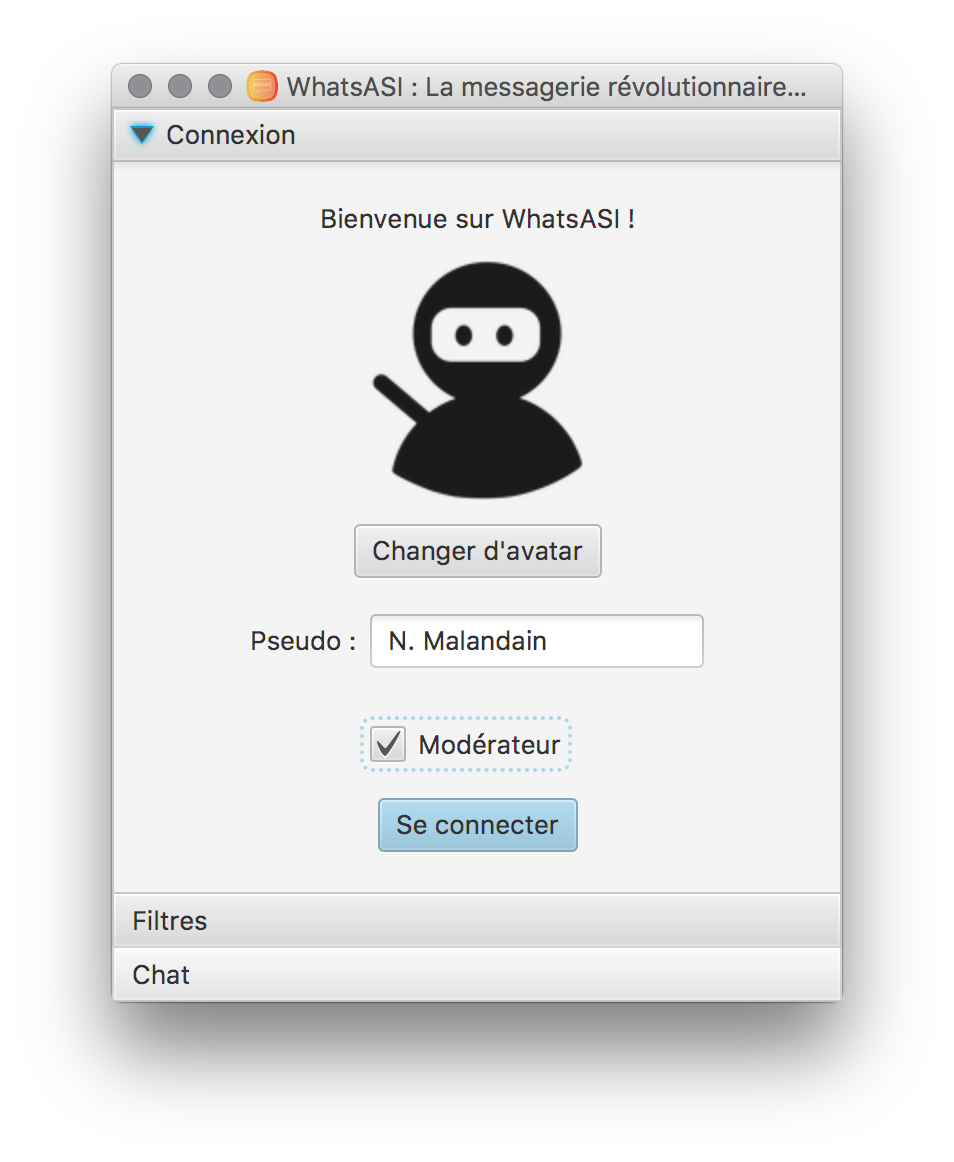
\includegraphics[width=0.5\textwidth]{images/illuConnexion.png}}
\end{figure}

\begin{figure}[H]
\caption{Panneau de filtrage}
\label{illuFiltre}
\centerline{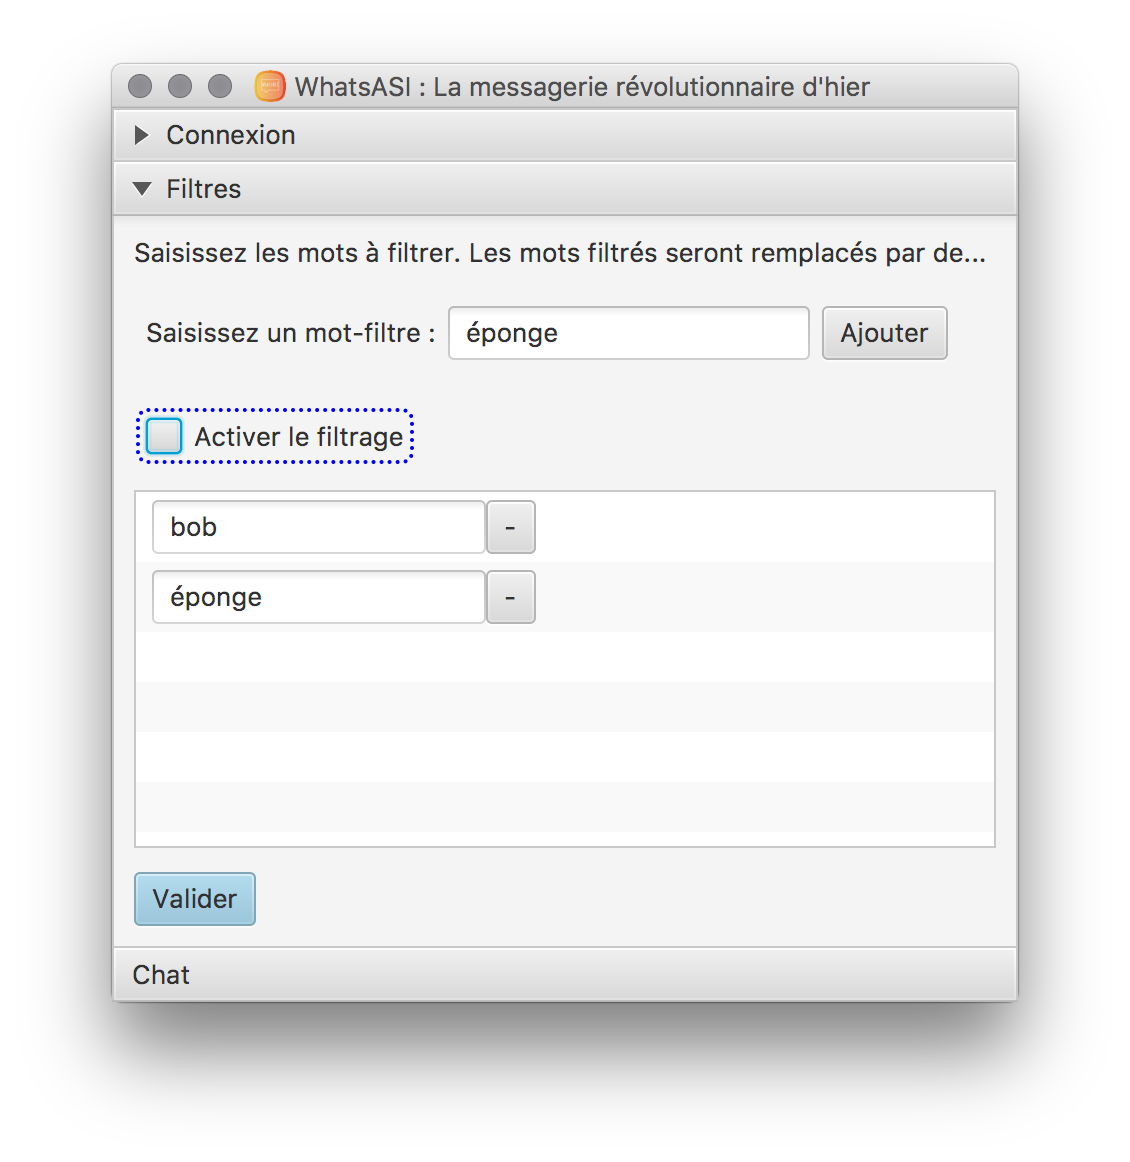
\includegraphics[width=0.5\textwidth]{images/illuFiltres.png}}
\end{figure}

\begin{figure}[H]
\caption{Panneau de conversation}
\label{illuConv}
\centerline{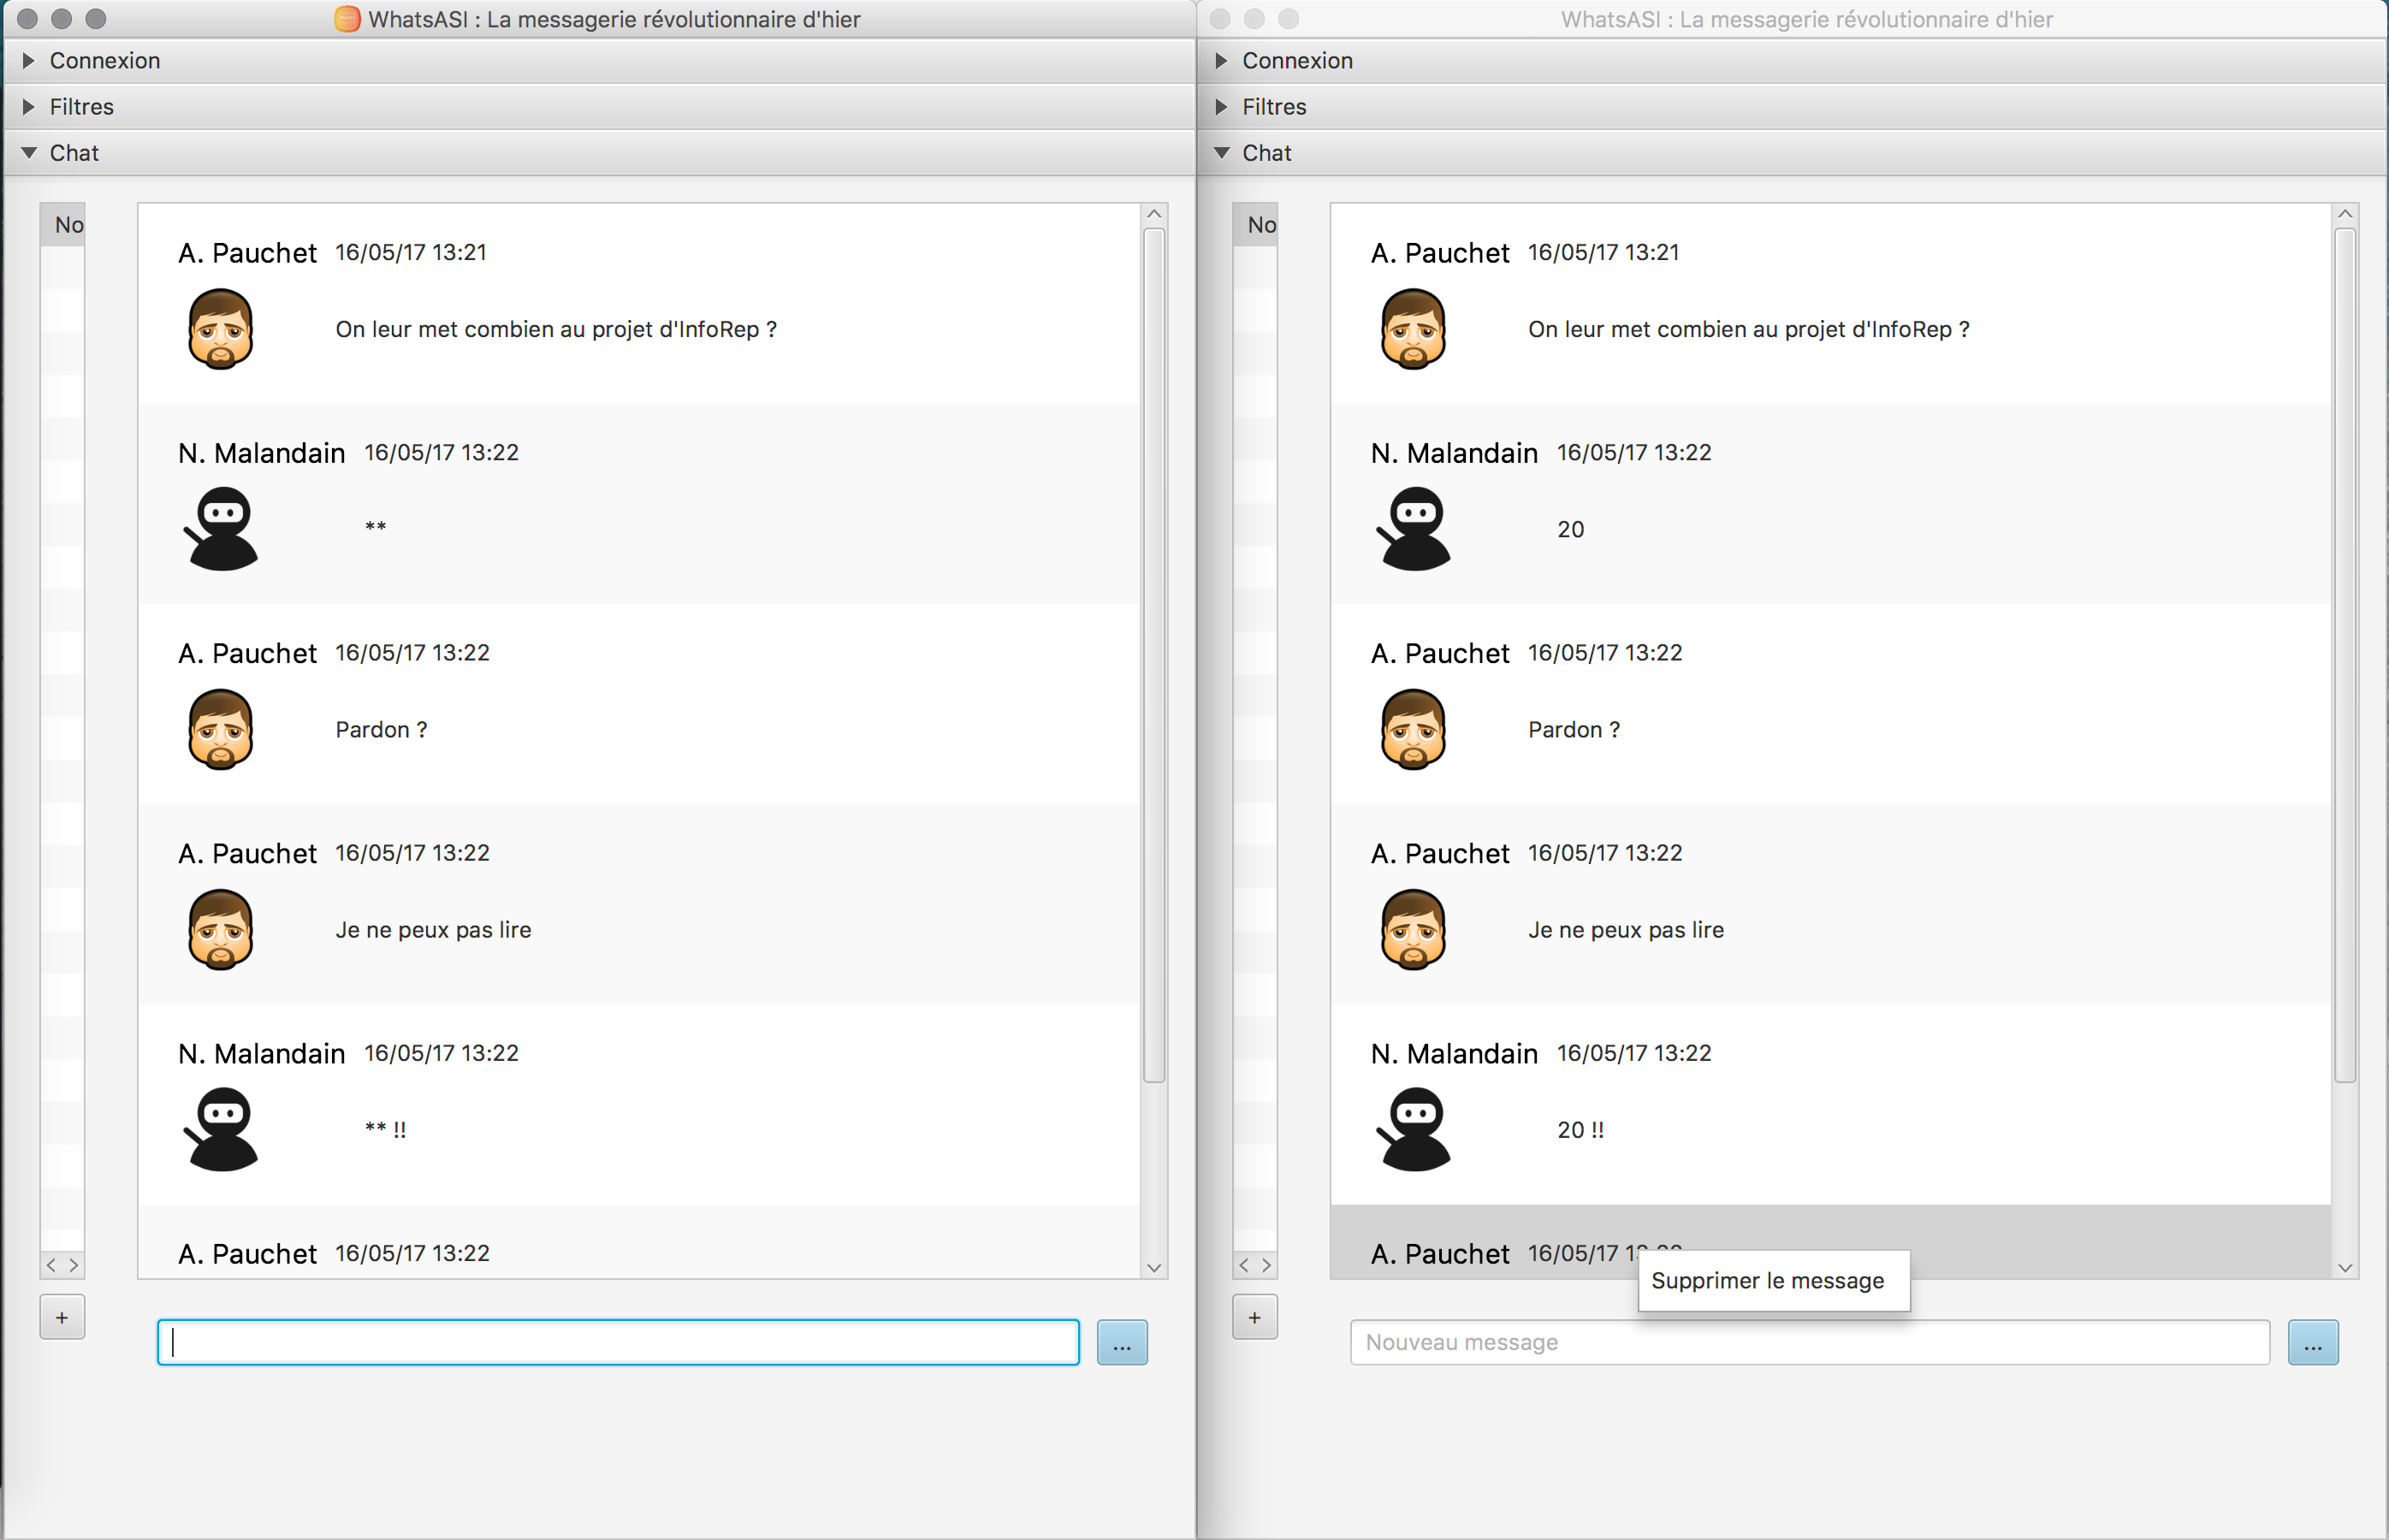
\includegraphics[width=1.2\textwidth]{images/illuConv.png}}
\end{figure}

\section{Tests de validation}
\subsection{Tests des spécifications fonctionnelles}
\begin{enumerate}
\item Les comptes utilisateurs ne persistent pas au-delà de la durée de vie d'un client de messagerie : OK
\item L'utilisateur peut paramétrer son compte, choisir un pseudo et un avatar : OK
\item Tout utilisateur peut rejoindre une conversation : OK
\item Les conversations persistent même quand aucun utilisateur n'y est actuellement connecté : OK
\item L'IA répond à toutes les commandes prévues : OK
\item Les modérateurs peuvent supprimer des messages et la suppression est propagée à la conversation et tous les utilisateurs : OK
\item Les mots à filtrer sélectionnés par un utilisateur sont filtrés dans toutes les conversations pour cet utilisateur seulement : OK
\end{enumerate}

\subsection{Tests des spécifications d'interface}
\begin{enumerate}
\item Il existe un panneau de connexion : OK
\item Il existe un panneau de filtrage : OK
\item Il existe un panneau de conversation où chaque message est affiché avec sa date, le pseudo et l'avatar de son expéditeur : OK
\item Une vue étendue s'affiche pour les conversations vidéos : KO (pas implémenté)
\item Les conversations audios sont supportées : KO
\end{enumerate}
\subsection{Tests des spécifications opérationnelles}
\begin{enumerate}
\item Le système de messagerie répond instantanément : OK
\item Les messages sont sauvegardés tant qu'il subsiste un utilisateur sur une conversation : OK (et plus longtemps encore)
\item Le service client est toujours accessible tant qu'est activé le serveur : OK
\item Chaque compte possède une référence propre : OK
\end{enumerate}

\chapter{Conclusion}
\section{Développement}
\subsection{Ce que nous avons développé}
\begin{enumerate}
\item Un serveur de messagerie hébergeant des conversations.
\item Un client graphique qui permet de créer un compte, filtrer des messages et participer à des conversations écrites.
\item Un client terminal.
\item Un helpbot.
\end{enumerate}
\subsection{Ce que nous avons abandonné}
La gestion de flux audio et flux vidéo.
Solution : utiliser un plugin permettant de gérer les flux audios et vidéos comme n'importe quel autre flux entre serveur et clients.
\section{Perspectives}
\begin{itemize}
\item Gérer les flux audios/vidéos.
\item Déployer un client Web.
\item Sécuriser le passage des références de compte au serveur avec un chiffrement asymétrique.
\end{itemize}



\end{document}
